\section{Experimental Evaluation}
\label{sec:exp}

We distinguish structural refresh cost, successful summary-token usage, and
measured graph-ready maintenance time. The first compares methods under the
abstract maintenance model; the latter two test whether less summary work
translates into lower token usage and elapsed update time in GraphRAG.
Graph-ready maintenance excludes raw-document extraction, and is distinct
from a full document-to-queryable update.
We study \textbf{(Q1)} graph-side maintenance latency and structural cost
against dynamic baselines; \textbf{(Q2)} implementation and selector overhead;
\textbf{(Q3)} the effects of batching and the exchange rate on work, delay,
and modularity (\S\ref{sec:exp:eff}); and \textbf{(Q4)} measured maintenance
time, update-summary tokens, and downstream synthesis quality
(\S\ref{sec:exp:e2e}). The graph-side timings below exclude LLM generation;
Exp-5 separately includes the summarization and publication stages.

\subsection{Experimental setup}
\label{sec:exp:setup}

% Both tables are queued here so that Table 3 fits this column and the
% wide Table 4 can take the top of the next page.
\begin{table}[b]\centering
\caption{Ten community-detection benchmarks.}
\label{tab:datasets}
\begin{footnotesize}
\setlength{\tabcolsep}{0.4em}
\begin{tabular}{lrrrrr}
\toprule
Dataset & $|V|$ & $|E|$ & avg.\ deg. & $Q$ & Batches \\
\midrule
Facebook    & $4{,}039$     & $88{,}234$      & $43.69$  & $0.835$ & $9$ \\
GPlus       & $107{,}614$   & $12{,}238{,}285$& $227.45$ & $0.475$ & $1{,}224$ \\
Twitter     & $81{,}306$    & $1{,}342{,}296$ & $33.02$  & $0.806$ & $135$ \\
Epinions    & $75{,}879$    & $405{,}740$     & $10.69$  & $0.441$ & $41$ \\
Cit-HepPh   & $34{,}546$    & $420{,}877$     & $24.37$  & $0.724$ & $43$ \\
Cit-HepTh   & $27{,}769$    & $352{,}285$     & $25.37$  & $0.656$ & $36$ \\
DBLP        & $317{,}080$   & $1{,}049{,}866$ & $6.62$   & $0.823$ & $105$ \\
Flickr      & $513{,}969$   & $3{,}190{,}452$ & $12.41$  & $0.665$ & $320$ \\
YouTube     & $1{,}134{,}890$&$2{,}987{,}624$ & $5.27$   & $0.722$ & $299$ \\
LiveJournal & $4{,}847{,}571$&$68{,}993{,}773$& $28.47$  & ---     & $6{,}900$ \\
\bottomrule
\end{tabular}
\par\smallskip\raggedright
$Q$: full-graph from-scratch \Louvain{}; Batches: $|\Delta E|=10^3$ updates
(LiveJournal: first $200$ evaluated).
\end{footnotesize}
\end{table}
% Compact Table 4: one column per retained dataset.
% Each cell reports Q / per-batch graph latency (ms) / abstract structural refresh cost.
\begin{table*}[t]
\centering
\caption{\textbf{Exp-1.} Modularity, latency, and structural re-summarization cost on ten graphs.}
\label{tab:main}
{\scriptsize
\setlength{\tabcolsep}{0.25pt}
\renewcommand{\arraystretch}{1.06}
\begin{tabular*}{\textwidth}{@{\extracolsep{\fill}}lcccccccccc@{}}
\toprule
Method & Facebook & Cit-Th & Cit-Ph & Epin. & Twitter & DBLP & GPlus$^*$ & Flickr$^*$ & YouTube$^*$ & LiveJ.$^{*\ddagger}$ \\
\midrule
\multicolumn{11}{l}{\emph{From-scratch, re-run per batch (cross-tool reference)}} \\
\Louvain{}
  & $.835/47.3/1.000$ & $.656/664/1.000$ & $.724/1021/1.000$
  & $.441/1380/1.000$ & $.806/\mathrm{TLE}/1.000$ & $.823/9753/1.000$
  & $.475/\mathrm{TLE}/1.000$ & $.665/\mathrm{TLE}/1.000$ & $.722/\mathrm{TLE}/1.000$ & $\text{--}/\text{--}/1.000$ \\
SLM
  & $.836/107/1.000$ & $.666/2854/1.000$ & $.737/3849/1.000$
  & $.454/4774/1.000$ & $.811/\mathrm{TLE}/1.000$ & $.837/25654/1.000$
  & $\mathrm{TLE}/\mathrm{TLE}/1.000$ & $.671/\mathrm{TLE}/1.000$ & $.733/\mathrm{TLE}/1.000$ & $\text{--}/\text{--}/1.000$ \\
Leiden
  & $.836/110/1.000$ & $.663/1880/1.000$ & $.734/2831/1.000$
  & $.445/4833/1.000$ & $.807/\mathrm{TLE}/1.000$ & $.828/21047/1.000$
  & $.477/\mathrm{TLE}/1.000$ & $.670/\mathrm{TLE}/1.000$ & $.732/\mathrm{TLE}/1.000$ & $.761/1332286/1.000$ \\
\midrule
Reuse-aware Leiden
  & $.836/285/.673$ & $.663/2275/.985$ & $.734/2841/.995$
  & $.445/2764/.964$ & $.807/6981/.980$ & $.828/19437/.996$
  & $.477^{\dagger}/66504^{\dagger}/\text{--}$ & $.670/28769/\text{--}$ & $.732/45397/\text{--}$ & $.761/\text{--}/.991$ \\
\DynaMo{}
  & $.836/15.7/.599$ & $.661/198/.982$ & $.722/269/.993$
  & $.452/249/.938$ & $.810/700/.957$ & $.827/2285/.989$
  & $.477/3739/.990$ & $.668/4091/.916$ & $.727/8721/.933$ & $.760/333821/.968$ \\
\Batch{}
  & $.835/101/.288$ & $.660/131/.899$ & $.732/131/.930$
  & $.435/169/.898$ & $.808/339/.579$ & $.822/475/.775$
  & $.475/4592/.479$ & $.665/1630/.802$ & $.722/2351/.935$ & $.750/28229/.834$ \\
\QCA{}
  & $.835/8.11/.452$ & $.661/10.4/.907$ & $.734/6.02/.934$
  & $.437/77.5/.825$ & $.808/9.79/.571$ & $.822/6.67/.711$
  & $.475/4973/.776$ & $.665/42.3/.705$ & $.722/75.2/.852$ & $.760/137/.773$ \\
DF-Leiden
  & $.835/4.51/.570$ & $.659/26.1/.981$ & $.730/35.4/.988$
  & $.442/39.5/.936$ & $.805/99.1/.763$ & $.823/212/.994$
  & $.476/690/.789$ & $.660/295/.844$ & $.719/560/.946$ & $.724/3555/.977$ \\
$\Delta$-screen
  & $.836/2.91/.330$ & $.656/13.0/.884$ & $.734/15.9/.923$
  & $.439/19.3/.861$ & $.782/61.4/.504$ & $.821/79.0/.693$
  & $.475/496/.393$ & $.658/186/.626$ & $.716/294/.842$ & $.731/595/.811$ \\
DF-\Louvain{}
  & $.835/2.24/.251$ & $.654/9.43/.883$ & $.731/11.5/.926$
  & $.438/13.9/.862$ & $.781/43.5/.527$ & $.819/54.6/.692$
  & $.475/380/.419$ & $.657/139/.628$ & $.713/213/.842$ & $.719/9.36/.846$ \\
\GreMod{}
  & $.835/2.22/.096$ & $.652/2.69/.204$ & $.727/2.74/.235$
  & $.434/3.44/.795$ & $.807/2.90/.185$ & $.820/4.88/.460$
  & $.475/4.89/.059$ & $.663/5.24/.674$ & $.720/8.10/.850$ & $.750/9.12/.629$ \\
HIT-Leiden
  & $.836/0.60/.275$ & $.665/6.95/.815$ & $.733/4.36/.875$
  & $.455/23.8/.875$ & $.811/14.6/.510$ & $.837/21.9/.742$
  & $.477/363/.482$ & $.667/111/.735$ & $.726/230/.883$ & $.768/217/.750$ \\
\midrule
\DyLo{}-\Louvain{}
  & $.835/0.39/.068$ & $.663/1.68/.051$ & $.730/1.60/.078$
  & $.445/3.97/.115$ & $.808/2.41/.080$ & $.820/4.36/.110$
  & $.471/3.43/.022$ & $.664/7.79/.037$ & $.718/20.5/.050$ & $.758/17.4/.010$ \\
\DyLo{}-SLM
  & $.836/0.39/.068$ & $.665/1.58/.051$ & $.735/1.65/.075$
  & $.452/3.82/.116$ & $.810/2.43/.077$ & $.831/4.16/.111$
  & $.477/3.70/.024$ & $.668/7.76/.037$ & $.724/21.6/.056$ & $.771/22.0/.010$ \\
\DyLo{}-Leiden
  & $.836/0.39/.069$ & $.666/1.59/.051$ & $.733/1.69/.091$
  & $.457/3.60/.117$ & $.811/2.43/.078$ & $.836/4.21/.113$
  & $.477/3.66/.026$ & $.668/7.89/.038$ & $.726/22.4/.056$ & $.768/21.2/.010$ \\
\bottomrule
\end{tabular*}
}
\begin{minipage}{\textwidth}
\scriptsize
Cells report five-run means where available of $Q$ / graph latency (ms per batch) / normalized
structural re-summarization cost, not token usage; $Q$ and cost are shown to
three decimals; $Q$ in the Epinions, Twitter, and DBLP columns is the stream mean of the runs in Figure~\ref{fig:qtrend}, except for \Louvain{}, SLM, \DyLo{}-\Louvain{}, and \DyLo{}-SLM. A complete reset costs $1.000$. All methods use the same
$r_{\mathrm{int}}=1$ structural metric, not fitted token weights. Structural
scores do not measure actual LLM execution or end-to-end latency. For the 18 \DyLo{} cells in the six unstarred
columns, the maximum seed range is
$3.3\times10^{-6}$ in $Q$ and $1.0\%$ relative to mean structural cost.
$*$: latency and structural cost come from separate measurement series.
$\ddagger$: LiveJournal, single run over the first $200$ batches; from-scratch \Louvain{} and SLM were not run. \textsc{tle}: time limit exceeded; $\dagger$: completed batches at
the time cap; \textbf{--}: not measured. All unmarked values cover the complete
update stream.
\end{minipage}
\end{table*}


\stitle{Environment.} \DyLo{}'s three instances and the four localized baselines
are implemented in C++17 (GCC~11.4,
\texttt{-O3 -march=native}); the four classic baselines use their released Java
implementations on OpenJDK~21. All runs are memory-resident and single-threaded
on Ubuntu~22.04 with an AMD EPYC~9654 and $1{,}128$\,GB RAM; Python~3.10 token
accounting is offline and never timed. The GraphRAG case study uses Qwen
for report generation and is separate from these CPU timing experiments.


\stitle{Datasets.} Table~\ref{tab:datasets} covers ten SNAP/Network Data
Repository benchmarks~\cite{snapnets,nr}: six social networks, one trust
network, two citation networks, and one co-authorship network. They span
diverse scales, densities, and community structures; DBLP and YouTube also
provide community metadata~\cite{yang2012groundtruth}. We treat vertices and
edges as already extracted entities and relations; directed inputs are
symmetrized and all ten graph workloads are undirected. MultiHop-RAG is a separate
workload-specific case study, not one of these ten benchmarks. On LiveJournal,
the largest graph, each evaluated method processes the first $200$ batches;
from-scratch \Louvain{} and SLM are not run there.

\stitle{Update streams.} We follow the standard protocol for dynamic community
detection~\cite{zhuang2019dynamo}: $90\%$ of the edges form the initial graph
and the remaining $10\%$ arrive as a stream. On the initial graph we build the
starting index---partition, hierarchy and per-node re-summarization
weights---by running the base detector once; every incremental method then
maintains its partition and hierarchy, whereas the rebuild baseline reruns the
base detector on the enlarged graph for every batch. The stream is cut into
batches of $|\Delta E|$ edges.
Unless stated otherwise $|\Delta E| = 10^3$.

\stitle{Competitors.} We evaluate four classic baselines---\DynaMo{}, \Batch{},
\GreMod{}, and \QCA{}---and four localized baselines---$\Delta$-screening,
DF-\Louvain{}, DF-Leiden, and HIT-Leiden---plus a \emph{reuse-aware rebuild}.
We also report from-scratch (FS) \Louvain{}, SLM, and Leiden references
(cross-tool $Q$; same-C++ latency); each resets the complete summary index and
therefore has cost $1$. The reuse-aware rebuild uses the same Leiden partition
as the corresponding FS Leiden reference, then matches new summary nodes to the
previous index by represented member set (or child set internally) and reuses
unchanged summaries. The two rows therefore share $Q$ and differ only in
rebuild latency and summary-reuse cost.

\stitle{Metrics and defaults.} We report stream-mean graph-maintenance
latency (excluding parsing, partition output, and LLM generation), modularity
$Q$, and normalized structural refresh cost under the abstract model.
Weights count entities at leaves and children internally; a complete reset
costs $1$. These scores are distinct from actual tokens and elapsed LLM time.
The paired deferral comparison additionally charges pending liabilities;
Exp-2 retains partition-derived structural scores. Accounting and timing
details are in Appendix~\ref{app:exp-defaults} and
Appendix~\ref{app:defer-seltime}.
Unless stated otherwise $\lambda=10^{-1}$. The main-table configuration
enables source deferral with $\varepsilon=0.05$. Table~\ref{tab:main}
reports five-run means where available; LiveJournal has one run. Exp-2
reports stream means from one recorded run per arm, and Exp-2b uses
three-seed medians. Starred columns combine separate latency and cost
measurements; dispersion and configuration details remain in the appendix.

\subsection{Maintenance efficiency}
\label{sec:exp:eff}

We first compare maintenance latency and structural refresh cost at the
reported modularity, then isolate the implementation and selection overheads.
Batch-size and exchange-rate sweeps examine how the savings trade off against
queueing delay and community quality.

% Single-column Exp-3 figure; defined before the wide Exp-4 float so that it
% keeps the number Figure 5.
\begin{figure}[tb]\centering
\includegraphics[width=\linewidth]{figures/exp3_batch.png}
\caption{\textbf{Exp-3.} Batching at $\lambda=0$: structural work per edge
versus approximate batch-closing delay (MH: MultiHop-RAG; HepPh: Cit-HepPh).}
\Description{Two log-log panels. Panel a plots re-summarization cost per edge
against batch size for eager and lazy evaluation on MultiHop-RAG and
Cit-HepPh, with queueing delay on a second axis rising with batch size. Panel
b plots the same costs against queueing delay, with points labeled by batch
size 1, 10, 100, and 1000.}
\label{fig:exp3}
\end{figure}

% Full-width float holding Exp-4 and Exp-2b (fig:knee).
\begin{figure*}[!tb]\centering
% Panels from scripts/make_fig_exp4_row.py.
\begin{subfigure}[t]{0.19\textwidth}\centering
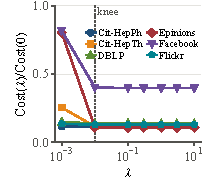
\includegraphics[width=\linewidth]{figures/exp4_cost.pdf}
\caption{Exp-4: cost.}
\end{subfigure}\hfill
\begin{subfigure}[t]{0.19\textwidth}\centering
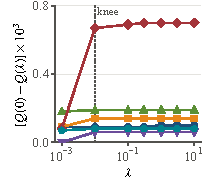
\includegraphics[width=\linewidth]{figures/exp4_qloss.pdf}
\caption{Exp-4: $Q$ loss.}
\end{subfigure}\hfill
\begin{subfigure}[t]{0.19\textwidth}\centering
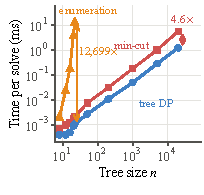
\includegraphics[width=\linewidth]{figures/exp2b_scaling.pdf}
\caption{Exp-2b: scaling.}
\end{subfigure}\hfill
\begin{subfigure}[t]{0.19\textwidth}\centering
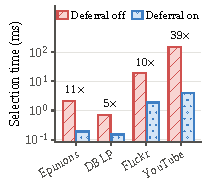
\includegraphics[width=\linewidth]{figures/exp2b_seltime.pdf}
\caption{Exp-2b: streams.}
\end{subfigure}\hfill
\begin{subfigure}[t]{0.19\textwidth}\centering
\includegraphics[width=\linewidth]{figures/gt_f1.pdf}
\caption{Answer $F_1$.}
\end{subfigure}
\caption{(a, b) \textbf{Exp-4.} Exchange-rate sensitivity (dotted: knee);
(c, d) \textbf{Exp-2b.} Selector time on synthetic trees ($n\le22$ binned) and
real streams with source deferral off/on; (e) token $F_1$ against reference
answers (FS: from-scratch).}
\Description{Five small panels. Panels a and b plot relative structural cost
and modularity loss against the exchange rate on a log axis for six graphs;
all curves flatten after a knee at 0.01. Panel c plots time per solve against
tree size on log-log axes: enumeration rises steeply and is 12,699 times
slower than tree DP at 22 nodes, while min-cut closure stays 1.7 to 4.6 times
slower than tree DP up to 20,000 nodes. Panel d compares deferral-off and
deferral-on selection time for Epinions, DBLP, Flickr, and YouTube, with
speedups of 11, 5, 10, and 39 times. Panel e shows token F1, with DyLo highest
at 0.187 and GreMod lowest at 0.089.}
\label{fig:knee}
\end{figure*}

\stitle{Exp-1: Against the baselines.} Table~\ref{tab:main} shows that
\DyLo{}-Leiden stays within $0.002$ of HIT-Leiden's rounded $Q$ on all ten
graphs, with reported graph-maintenance speedups of about
$1.5$--$99\times$ and structural cost about $75$--$99\%$ lower.
Across the three \DyLo{} instances, each has lower structural cost than every
incremental baseline on all ten graphs. Where a corresponding from-scratch
reference is available, the reported $Q$ is at most $0.01$ lower; the
row-specific aggregation conventions are stated in the table notes.
This is a trade-off rather than universal latency dominance: \GreMod{} is
faster on Epinions, Flickr, YouTube, and LiveJournal, and DF-\Louvain{} is
faster on LiveJournal, at lower $Q$ and higher structural cost. Where both
costs are available, reuse-aware rebuild costs about $8$--$99\times$ as much
as \DyLo{}-Leiden. On LiveJournal, \DyLo{}-Leiden matches HIT-Leiden's
rounded $Q$ with $0.010$ versus $0.750$ structural cost. The starred columns
support descriptive comparisons across measurement series, rather than
paired latency--cost measurements.

\begin{figure}[tb]\centering
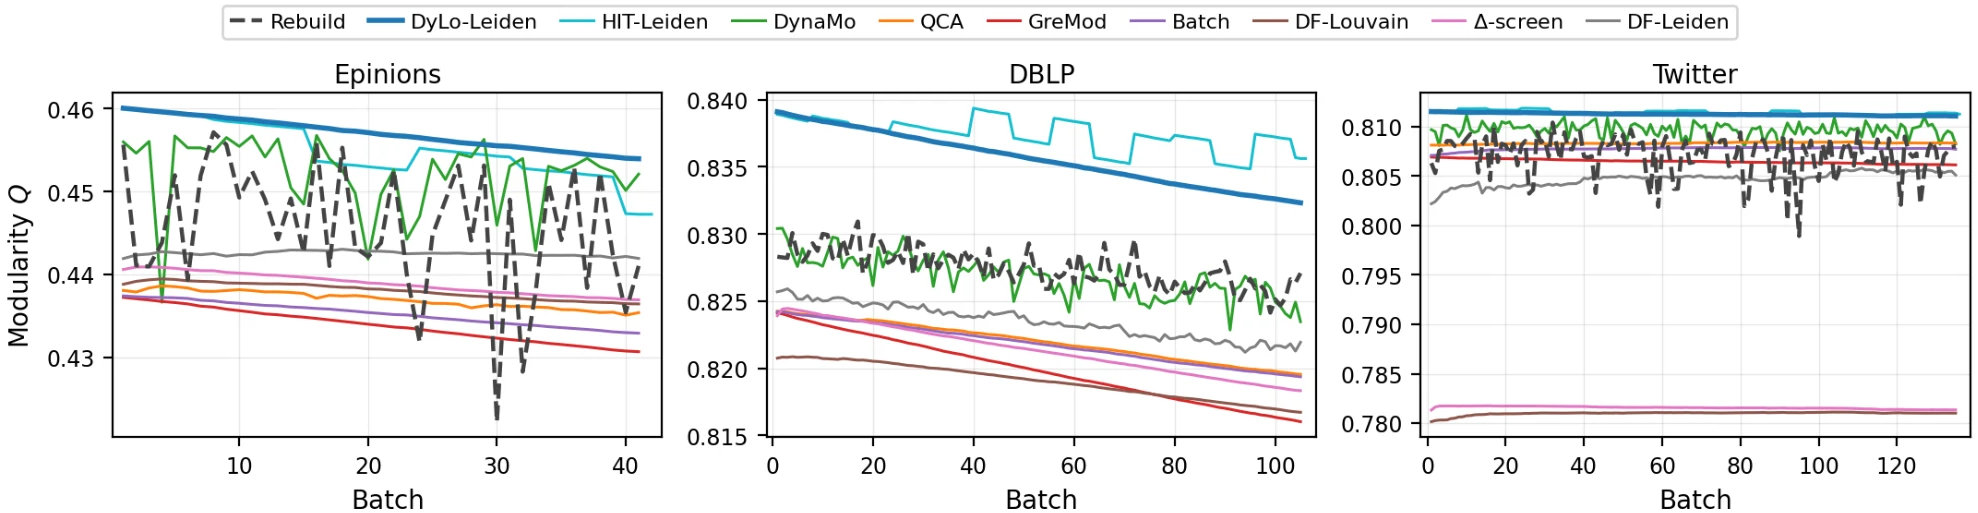
\includegraphics[width=\linewidth]{figures/q_trend.png}
\caption{\textbf{Exp-1.} Per-batch modularity $Q$ along the update stream
(Rebuild: Leiden rerun on each batch).}
\Description{Three line charts side by side of modularity against batch index
for Epinions, DBLP, and Twitter, one line per method, with a shared legend on
top. DyLo-Leiden and HIT-Leiden are on top in every panel; the dashed rebuild
line fluctuates strongly; GreMod is near the bottom.}
\label{fig:qtrend}
\end{figure}

\stitle{Quality along the stream.} On the three plotted streams,
Epinions, DBLP, and Twitter (Figure~\ref{fig:qtrend}), \DyLo{}-Leiden's
per-batch $Q$ is at most $0.005$ below HIT-Leiden's. The rebuild fluctuates
more while restarting the detector at each batch. These observations support
small modularity losses on the evaluated streams; they do not establish
answer quality, which we examine separately.

\begin{table}[tb]
\centering
\caption{\textbf{Exp-2.} Component ablation (one run per arm; stream means).}
\label{tab:ablation}
\begin{scriptsize}
\setlength{\tabcolsep}{0.25em}
\begin{tabular*}{\linewidth}{@{\extracolsep{\fill}}clrrc@{}}
\toprule
Variant & Removed & Latency (ms) & Struct. cost & Commit \\
\midrule
$V_0$ & ---          & $4.72/9.60/27.4$ & $.133/.046/.057$ & --- \\
\midrule
$V_1$ & certificates & $11.4/17.4/43.5$ & $.133/.046/.057$ & same \\
$V_2$ & cost tree    & $6.07/15.9/57.9$ & $.133/.046/.057$ & same \\
$V_3$ & pruning      & $7.66/13.0/39.3$ & $.144/.050/.061$ & changed \\
\bottomrule
\end{tabular*}
\par\smallskip\raggedright
Triplets: Epinions/Flickr/YouTube. Cost is reconstructed from per-batch
partitions. Every arm has rounded $Q=.4559/.6692/.7277$.
\end{scriptsize}
\end{table}

\stitle{Exp-2: Implementation speedups.}
Table~\ref{tab:ablation} removes one optimization at a time
($V_0$ is an internal control). Removing certificates raises measured
latency to $1.59$--$2.42\times$ the control; removing incremental cost-tree
maintenance raises it to $1.29$--$2.11\times$. Both preserve the recorded partitions
and structural scores, supporting their role in avoiding repeated work. Pruning also reduces latency and cost while changing the committed sets
at the reported $Q$. Safe pruning preserves the frozen problem's optimum
value, not a unique maximizer or the subsequent trajectory; these different
costs therefore do not by themselves demonstrate a better frozen optimum.
These single-run timings are descriptive; the internal control and its
partition-derived cost should be compared within this ablation.

\stitle{Certified frontier in practice.} On nine graphs over the first
$40$ batches (or the full shorter stream), a batch of $10^3$ edges
re-examines a median of only $2$--$277$ vertices. Certificate checks skip
re-examination $99.1$--$100\%$ of the time, with at most $18$ expirations per
batch on average. These windows support observed locality, not a worst-case
bound or a result on LiveJournal; the live certificate store grows with
graph size. Per-graph statistics are in Appendix~\ref{app:frontier}.

% Integrated from the author-supplied experiment, 2026-09-24.
% Author clarified: 5,000 total small-instance comparisons; same environment
% and timing scope as the manuscript. Original preserved under output/.
\stitle{Exp-2b: Exact selection through the single-anchor reduction.}
\label{sec:exp:selector}
We ask whether the tree solver is exact and fast, and how the single-anchor
configuration affects selection on real streams.

\emph{Same-instance exactness and scaling.}
On synthetic forests with the node objective of Theorem~\ref{thm:dp} (gains from
$U(-10,10)$, $\lambda\in\{0,0.1,0.5,1,2\}$), we compare exhaustive enumeration,
generic maximum-weight closure~\cite{picard1976maximal} solved by min-cut, and
tree DP.

All three solvers return identical selections in all $5{,}000$ enumerable
tests, and DP and closure still agree up to $20{,}000$ nodes.
Figure~\ref{fig:knee}(c) shows DP to be the fastest at every size:
enumeration explodes beyond $20$ nodes, and closure stays slower throughout,
with a gap that widens as trees grow (timings in
Appendix~\ref{app:defer-seltime}).


\emph{Real-stream selection.}
Without deferral, two-anchor actions use min-cut while single-anchor rounds
can use DP; with deferral, all $2{,}079$ reported rounds use DP.
Figure~\ref{fig:knee}(d) labels these configurations as \emph{Deferral off}
and \emph{Deferral on} and compares full-stream selection totals, with up to
$39\times$ reduction on YouTube. This is a configuration comparison, not
a matched-input solver comparison or a $39\times$ overall speedup:
YouTube driver latency changes from $27.2$ to $26.9$\,ms per batch.
Timing boundaries and per-graph values are in Appendix~\ref{app:defer-seltime}.

In the separate schedule-plus-closing-balance comparison, cumulative accrual
cost agrees on $23$ of $24$ graph--instance pairs and is $0.01\%$ higher on
the last, with $Q$ agreeing to five decimals. Deferred work is charged rather
than counted as free; the observed effect is nearly unchanged total cost.


\stitle{Selector fidelity.} Validation accepted all $1{,}437$ nonempty groups
the surrogate proposed across eight graphs and three instances, and
\textsc{Peel} never fired. This is an empirical acceptance result for those
groups. Per-destination greedy selection matches the tree DP at the
default rate. At smaller rates, DP can exploit shared ancestor costs:
the recorded objective gain reaches about $100\%$ on Epinions, with
smaller gains on other graphs. At the default working point, the measured
benefit of the single-anchor reduction is chiefly lower selection time.

% Temporarily hidden (2026-09-23): Exp-2c is not required for the
% single-anchor / exact-DP contribution. Preserve the source for restoration.
% \input{tabepssweep}

\stitle{Exp-3: Batch size and batch-closing delay.}
\label{sec:exp:batch}
We replay MultiHop-RAG and Cit-HepPh with batch sizes
$E\in\{1,10,100,1000\}$ (Figure~\ref{fig:exp3};
Appendix~\ref{app:exp3-detail}). At the measured extraction rate of $6.04$
edges/s, the plotted batch-closing delay uses the approximation
$E/(2\cdot6.04)$\,s; it excludes subsequent maintenance and summary generation.
The figure reports unnormalized structural weight per edge at $\lambda=0$:
larger batches amortize work but increase waiting. At the default priced
rate, MultiHop-RAG singleton processing already costs $0.611$ per edge
(not plotted; $113.5$ without pricing). Lazy evaluation further reduces
singleton work when updates are localized, as on Cit-HepPh.

\stitle{Exp-4: Sensitivity to the exchange rate.}
Figure~\ref{fig:knee}(a, b) sweeps $\lambda$ on six graphs, reporting
$\mathrm{Cost}(\lambda)/\mathrm{Cost}(0)$ and $Q(0)-Q(\lambda)$.
The recorded curves flatten beyond $\lambda=10^{-2}$, after large
reductions in structural work at small modularity loss; Facebook benefits
less. We use the shared default $\lambda=10^{-1}$ instead of tuning per graph
(Appendix~\ref{app:exp4-detail}). The reference is the same sweep's
$\lambda=0$ run, not the separate from-scratch detector; frozen-round
monotonicity does not imply monotonicity across stream trajectories.

\subsection{Case study: Maintenance efficiency and sensemaking quality}
\label{sec:exp:e2e}

\begin{comment}

\stitle{Exp-6 \& Exp-7: Token cost and answer quality on HotpotQA.} We evaluate a HotpotQA~\cite{yang2018hotpotqa} GraphRAG index under a $20$-batch stream (Table~\ref{tab:tokens}), measuring the input tokens of every regenerated summary.

\emph{Token cost.} \DyLo{}-Leiden regenerates $51.8$k input tokens per batch, $83.7\%$ fewer than from-scratch. DF-\Louvain{} and $\Delta$-screen appear inexpensive partly because more than $82\%$ of their communities remain unchanged; \DyLo{} retains only $29.5\%$ unchanged yet still regenerates the fewest tokens by selecting cheaper communities.

\begin{table}[tb]\centering
\caption{\textbf{Exp-7.} LLM input tokens per batch on the HotpotQA index
(GPT-4o-mini input rate: \$0.15/M~\cite{openai2024gpt4omini}); the lower block reports answer quality on the same index.}
\label{tab:tokens}
\begin{footnotesize}
\setlength{\tabcolsep}{0.35em}
\resizebox{\linewidth}{!}{%
\begin{tabular}{lrrrrr}
\toprule
Method & Unch.\ (\%) & Comms/b. & Tokens/b. & \$/b. & Saved (\%) \\
\midrule
From-scratch Leiden & --- & $826$ & $317{,}662$ & $0.0476$ & --- \\
\midrule
\DynaMo{}       & $71.9$ & $118$ & $147{,}798$ & $0.0222$ & $53.5$ \\
DF-Leiden       & $72.9$ & $98$  & $125{,}388$ & $0.0188$ & $60.5$ \\
HIT-Leiden      & $20.6$ & $225$ & $111{,}063$ & $0.0167$ & $65.0$ \\
\GreMod{}       & $53.6$ & $127$ & $90{,}379$  & $0.0136$ & $71.5$ \\
\QCA{}          & $39.7$ & $96$  & $82{,}146$  & $0.0123$ & $74.1$ \\
\Batch{}        & $75.0$ & $64$  & $74{,}563$  & $0.0112$ & $76.5$ \\
$\Delta$-screen & $82.5$ & $54$  & $72{,}698$  & $0.0109$ & $77.1$ \\
DF-\Louvain{}   & $\mathbf{82.6}$ & $45$ & $59{,}696$ & $0.0090$ & $81.2$ \\
\midrule
\DyLo{}-Leiden  & $29.5$ & $322$ & $\mathbf{51{,}827}$ & $\mathbf{0.0078}$ & $\mathbf{83.7}$ \\
\midrule
\multicolumn{6}{l}{\emph{Answer quality on the same index ($306$ questions)}} \\
\cmidrule(lr){1-6}
Index & Unch.\ (\%) & $F_1$ & EM & UNKNOWN & W/L/T \\
\midrule
All-fresh         & ---    & $.0769$ & $.0490$ & $79.7\%$ & --- \\
\DyLo{}           & $29.5$ & $\mathbf{.0817}$ & $\mathbf{.0523}$ & $\mathbf{78.4\%}$ & $5/4/297$ \\
Mask-$40$ control & ---    & $.0444$ & $.0327$ & $87.9\%$ & $22/9/275$ \\
\bottomrule
\end{tabular}}
\end{footnotesize}
\end{table}

\emph{Answer quality.} Against the same partition with every summary refreshed, \DyLo{}'s selective index is statistically indistinguishable over $306$ questions (paired token-$F_1$ $\Delta=-.0047$, $95\%$ CI $[-.016,+.007]$; $5/4/297$, $p=1.000$). In contrast, blanking $40\%$ of summaries reduces token-$F_1$ by $.0326$ ($p=.029$), showing that the evaluation detects semantic loss but no penalty from \DyLo{}'s selective deferral.
\FloatBarrier

\end{comment}

\stitle{Structural cost and token usage.} Count-based structural weights
approximate summary size imperfectly, especially at internal nodes
(Appendix~\ref{app:proxy-cal}). We therefore measure actual update-summary
tokens and maintenance time separately in Exp-5.

\stitle{Exp-5: Measured maintenance and sensemaking quality.}
We update a MultiHop-RAG~\cite{tang2024multihoprag} index from $304$ to $327$
articles, using the same extracted graph and
Qwen2.5-7B-Instruct~\cite{yang2024qwen25} report generator across eight arms.
Incremental arms reuse reports with unchanged community membership;
Rebuild regenerates all reports. Each arm runs alone on an H100.
Appendix~\ref{app:exp5-detail} details the original \texttt{std4} replay
and accounting.

\begin{table}[tb]\centering
\caption{\textbf{Exp-5.} Measured maintenance on the same $304\!\to\!327$-document graph.}
\label{tab:arena-main}
\footnotesize
\setlength{\tabcolsep}{0.25em}
\begin{tabular*}{\linewidth}{@{\extracolsep{\fill}}lrrrrr@{}}
\toprule
Method & Calls & $T_s$ (s) & $T_s/T_m$ (\%) & Tok. (k) & $T_m$ (s) \\
\midrule
Rebuild & 1637 & 2116.1 & 98.7 & 2,965.9 & 2144.7 \\
HIT-Leiden & 721 & 934.9 & 97.3 & 1,601.6 & 961.1 \\
\DynaMo{} & 717 & 948.8 & 97.3 & 1,616.1 & 974.8 \\
\QCA{} & 695 & 936.7 & 97.2 & 1,558.3 & 963.1 \\
DF-\Louvain{} & 717 & 964.7 & 97.4 & 1,628.9 & 990.8 \\
$\Delta$-screen & 732 & 960.9 & 97.4 & 1,653.7 & 987.0 \\
\Batch{} & 712 & 931.3 & 97.2 & 1,588.9 & 957.9 \\
\DyLo{} & $\mathbf{344}$ & $\mathbf{521.7}$ & $\mathbf{95.2}$ & $\mathbf{1,157.2}$ & $\mathbf{547.9}$ \\
\bottomrule
\end{tabular*}
\par\smallskip\raggedright
$T_s$: summarization time; $T_m$: graph-ready to queryable maintenance.
Calls and tokens count successful update summaries (native input plus output).
Initial construction, extraction, and old-report repair are excluded; retry
time is included. One run per arm.
\end{table}

\emph{Maintenance savings.} Re-summarization accounts for $95.2$--$98.7\%$
of graph-ready maintenance time, while community detection takes less than
$0.2\%$ (Table~\ref{tab:arena-main}; Appendix~\ref{app:exp5-detail}).
Reducing summary refreshes therefore targets the dominant bottleneck.
By regenerating fewer reports, \DyLo{} reduces update-summary tokens by
$27.2\%$ versus \Batch{} and $61.0\%$ versus Rebuild, with corresponding
maintenance-time reductions of $42.8\%$ and $74.5\%$.

\emph{Sensemaking quality.} We evaluate the first $60$ archived synthesis
questions ($q_0$--$q_{59}$)
with GraphRAG global search~\cite{edge2024graphrag}, using each index's
complete root-report cut. An independent local \texttt{gpt-oss-120b} judge
compares anonymized answers in both orders on comprehensiveness, diversity,
empowerment, and directness.

\begin{table}[tb]\centering
\caption{\textbf{Exp-5.} DyLo preference against each baseline on $60$ synthesis questions ($\uparrow$).}
\label{tab:sensemaking-current}
\footnotesize
\setlength{\tabcolsep}{0.25em}
\begin{tabular*}{\linewidth}{@{\extracolsep{\fill}}lrrrr@{}}
\toprule
Opponent & Comp. & Div. & Emp. & Dir. \\
\midrule
\Batch{} & 60.00 & 66.25 & 53.33 & 49.58 \\
Rebuild & 56.67 & 61.25 & 48.33 & 48.33 \\
HIT-Leiden & 57.50 & 62.08 & 51.67 & 57.50 \\
\DynaMo{} & 64.17 & 63.75 & 52.50 & 55.00 \\
\QCA{} & 69.58 & 75.83 & 53.75 & 53.75 \\
DF-\Louvain{} & 55.00 & 56.25 & 52.50 & 47.08 \\
$\Delta$-screen & 53.33 & 60.83 & 48.75 & 40.00 \\
\bottomrule
\end{tabular*}
\par\smallskip\raggedright
Win/tie/loss scores are $100/50/0$, averaged over both answer orders;
$50$ denotes equal preference. Question-bootstrap intervals and order
sensitivity are in Appendix~\ref{app:exp5-detail}.
\end{table}

\DyLo{}'s comprehensiveness and diversity point scores exceed $50$ against
all seven baselines. Diversity scores against \Batch{} and Rebuild have
unadjusted $95\%$ intervals above $50$, while empowerment and directness
are mixed; directness falls to $40.00$ against $\Delta$-screen.
Thus maintenance savings coexist with favorable synthesis preferences
but no uniform quality advantage; native report exposure also differs
across partitions.

\emph{Implication for full updates.} With common upstream extraction,
full-update savings equal $f_m r_m$, where $r_m$ is the relative maintenance
reduction and $f_m$ is maintenance's share of baseline time. The benefit
is greatest when maintenance dominates; full-update speedups were not measured.


\stitle{Reference-answer check.}
On a separate $609$-article, $20$-batch stream, \DyLo{}-Leiden has the highest
token-$F_1$ point estimate across $414$ final-snapshot questions
(Figure~\ref{fig:knee}(e)). Unadjusted paired $95\%$ intervals support gains over
from-scratch Leiden, \Batch{}, \DynaMo{}, and \GreMod{}; comparisons with
\QCA{} and from-scratch \Louvain{} remain inconclusive
(Appendix~\ref{app:groundtruth}).

% Temporarily hidden at the author's request, 2026-09-24.
\begin{comment}
\begin{table}[!htbp]\centering
\caption{Reference-answer freshness controls.}
\label{tab:mhrag-controls}
\begin{footnotesize}
\setlength{\tabcolsep}{0.7em}
\begin{tabular}{lrr}
\toprule
Check & Token-$F_1$ change & $p$ \\
\midrule
Selective deferral & $|\Delta F_1|=.0007$ & $1.000$ \\
Mask-$40$ blanking & $\Delta F_1=-.0644$ & $<10^{-3}$ \\
\bottomrule
\end{tabular}
\end{footnotesize}
\end{table}

Table~\ref{tab:mhrag-controls} detects the loss from summary blanking but no
significant difference between selective deferral and its fresh-summary
control. This establishes measurement sensitivity and complements the arena's
open-ended synthesis test.
\end{comment}
\FloatBarrier

